\chapter{\label{capterParabolicOptimalControlProblems}Parabolic optimal control problems}

\section{Introduction to the problem}
Our optimization problem is based on the problem that is presented in \cite{doi:10.1137/070694016}. We consider a state variable $u$ and a control variable $q$, defined on $(0,T)\times\Omega$ with $T\in\mathbb{R}$ and $\Omega\subset\mathbb{R}^n$.

The goal of this thesis is to minimize the functional
\begin{subequations}
\label{conProb}
\begin{gather}
J(q,u)=\frac{1}{2}\int_0^T\int_\Omega(u(t,x)-\hat{u}(t,x))^2\,\mathrm{d}x\,\mathrm{d}t+\frac{\alpha}{2}\int_0^T\int_\Omega q(t,x)^2\,\mathrm{d}x\,\mathrm{d}t\label{objFun},\\
%\end{equation}
\intertext{subject to the constraints}
%\begin{equation}
\begin{aligned}
	\partial_tu-\Delta u&=f+q&\text{ in }(0,T)\times\Omega,\\
	u(0)&=u_0&\text{ in }\Omega,
\end{aligned}
\label{constraints}
\end{gather}
\end{subequations}
with homogeneous Dirichlet boundary conditions on $(0,T)\times\partial\Omega$.

Let $V=H_0^1(\Omega)$, $H=L^2(\Omega)$ and $I=(0,T)$. We define our state space as
\begin{displaymath}
X:=\{v\mid v\in L^2(I,V)\text{ and }\partial_tv\in L^2(I,V^*)\}
\end{displaymath}
and the control space as
\begin{displaymath}
Q:=L^2(I,L^2(\Omega)).
\end{displaymath}
The notion of the inner products and norms on $L^2(\Omega)$ and $L^2(I,L^2(\Omega))$ is introduced as
\begin{align*}
(v,w)&:=(v,w)_{L^2(\Omega)},&(v,w)_I&:=(v,w)_{L^2(I,L^2(\Omega))},\\
\|v\|&:=\|v\|_{L^2(\Omega)},&\|v\|_I&:=\|v\|_{L^2(I,L^2(\Omega))}.
\end{align*}
By using the inner product, the weak form of the state equations \eqref{constraints} for $q,f\in Q$ and $u_0\in V$ is given as
\begin{equation}
\label{weakEq}
\begin{aligned}
	(\partial_tu,\phi)_I+(\nabla u,\nabla\phi)_I&=(f+q,\phi)_I&\forall\phi\in X,\\
	u(0)&=u_0&\text{ in }\Omega.
\end{aligned}
\end{equation}
With the weak state equations \eqref{weakEq}, we define the weak formulation of the optimal control problem \eqref{conProb} as
\begin{equation}
\label{weakProb}
\text{Minimize }J(q,u):=\frac{1}{2}\|u-\hat{u}\|_I^2+\frac{\alpha}{2}\|q\|_I^2\text{ subject to \eqref{weakEq} and }(q,u)\in Q\times X.
\end{equation}

Now we cite two results of the problems \eqref{weakEq} and \eqref{weakProb} from \cite{doi:10.1137/070694016}.

\begin{prop}[\cite{doi:10.1137/070694016}]
\label{uniqueU}
For fixed $q,f\in Q$, and $u_0\in V$ there exists a unique solution $u\in X$ of problem \eqref{weakEq}. Moreover, the solution exhibits the improved regularity
\begin{displaymath}
u\in L^2(I,H^2(\Omega)\cap V)\cap H^1(I,L^2(\Omega))\hookrightarrow C(\bar{I},V).
\end{displaymath}
It holds the stability estimate
\begin{displaymath}
\|\partial_tu\|_I+\|\nabla^2u\|_I\leq C\{\|f+q\|_I+\|\nabla u_0\|\}.
\end{displaymath}
\end{prop}

%evtl rauslassen
\begin{prop}[\cite{doi:10.1137/070694016}]
For given $f,\hat{u}\in L^2(I,H)$, $u_0\in V$, and $\alpha>0$, the optimal control problem \eqref{weakProb} admits a unique solution $(\bar{q},\bar{u})\in Q\times X$. The optimal control $\bar{q}$ posesses the regularity
\begin{displaymath}
\bar{q}\in L^2(I,H^2(\Omega))\cap H^1(I,L^2(\Omega)).
\end{displaymath}
\end{prop}

Due to the existence and uniqueness results from Proposition \ref{uniqueU}, we define $u(q)$ as the unique solution of \eqref{weakEq} with respect to some $q\in Q$. This enables us to define a reduced cost functional $j:Q\to \mathbb{R}$ that is only dependent on the control $q$ as
\begin{displaymath}
j(q):=J(q,u(q)).
\end{displaymath}
From now on, the optimal control problem that we examine is:
\begin{equation}
\label{redProb}
\text{minimize }j(q)\text{ subject to }q\in Q.
\end{equation}

\section{Finite element discretization}
In order to solve the optimization problem \eqref{redProb} numerically, the discretization of our model is now discussed. We use finite elements methods \cite{doi:10.1137/1.9780898717440, articleMeidner} for this. At first, the discretization in space with a n-D continuous Galerkin method is presented. Then, we look at the discretization in time, which is done with a 1D continuous Galerkin method. From now on, we will also discuss some implementation details, so in this chapter how we handle the calculation of the objective function $j$. In our implementation, we apply functions from the Python package pyMOR.

\subsection{\label{SubsectionDiscretizationInSpace}Discretization in space}
The discretization in space is shown on a 2-dimensional rectangular space $\Omega\subset\mathbb{R}^2$ with linear finite elements. We assume to have a vertex set $\mathcal{V}=(x_1,\dotsc,x_{N_\mathcal{V}})\in(\mathbb{R}^2)^{N_\mathcal{V}}$ with a convex hull that is equal  to $\bar{\Omega}$ and $x_i\neq x_j$ for all $i\neq j$ in $\{1,\dotsc,N_\mathcal{V}\}$. Let $\hat{T}=\{(x,y)\in[0,1]^2\mid y \leq 1-x\}$ be the reference triangle. Then,
\begin{displaymath}
\theta_l(\xi)=x_{l_1} + D\theta_l \begin{pmatrix} \xi_1 \\ \xi_2 \end{pmatrix} \text{ with } D\theta_l = \begin{pmatrix} x_{l_2}-x_{l_1} & x_{l_3}-x_{l_1} \end{pmatrix}
\end{displaymath}
is a transformation from the reference triangle $\hat{T}$ to some other triangle $T_l$ with the corners $x_{l_1}, x_{l_2}, x_{l_3}\in\mathcal{V}$.

We define now a mesh $\mathcal{T}=\{T_l\}$ which consists of triangles $T_l=\theta_l(\hat{T})$, where $T_l\cap T_m$ for $T_l,T_m\in\mathcal{T}$ is either a common side, a common corner, or empty, and where $\bar{\Omega}=\cup_{T_l\in\mathcal{T}}T_l$. We also assume that every vertex in $\mathcal{V}$ is a corner of at least one triangle of $\mathcal{T}$.\\

With pyMOR functions, we discretize a rectangular domain by specifying the number of grid intervals first. Then, the domain is subdivided into smaller rectangles of the same size, so that the number of rectangles along the $x$- and the $y$-axis is equal to the predefined number of grid intervals. Each smaller rectangular unit is then partitioned into four equally sized triangles by adding a vertex into the center of the rectangle which is connected with the corners of the unit. The vertex set of the whole domain is now given by the union of the corners of all triangles. As an example, if a domain $\Omega = [a, a]$ with $a>0$ is given and we set the number of grid intervals to two, then our mesh would look like that:
\begin{figure}
    \centering
    %\textbf{Your title}\par\medskip
    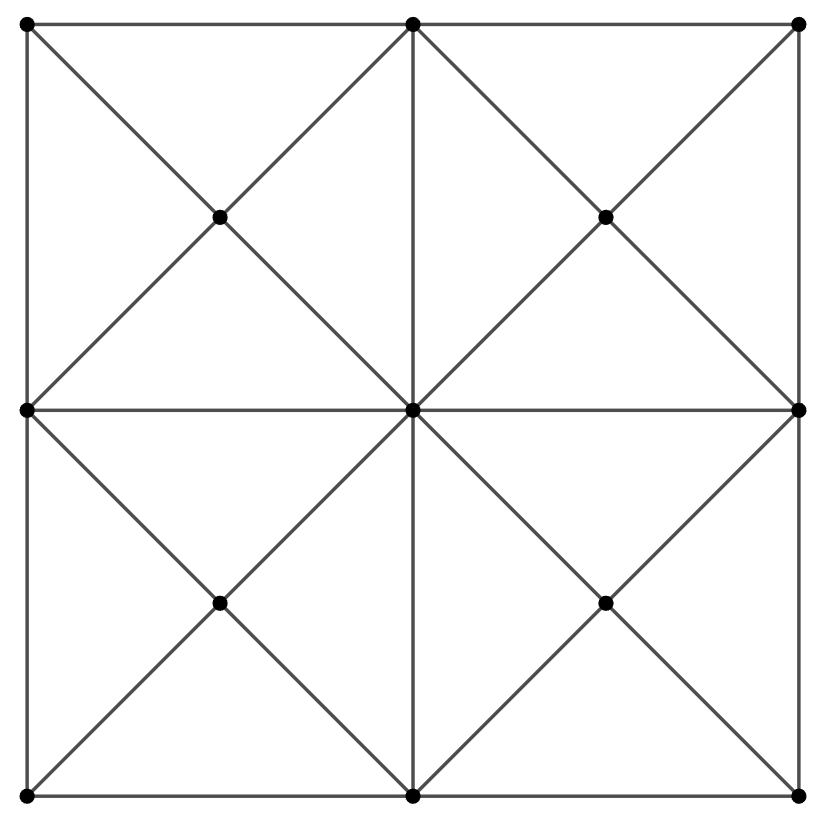
\includegraphics[height=8cm]{mesh.png} 
    \caption{Example of a mesh with two grid intervals in a square-shaped domain. The dots denote elements of the vertex set $\mathcal{V}$.}
\end{figure}
%\begin{center}
%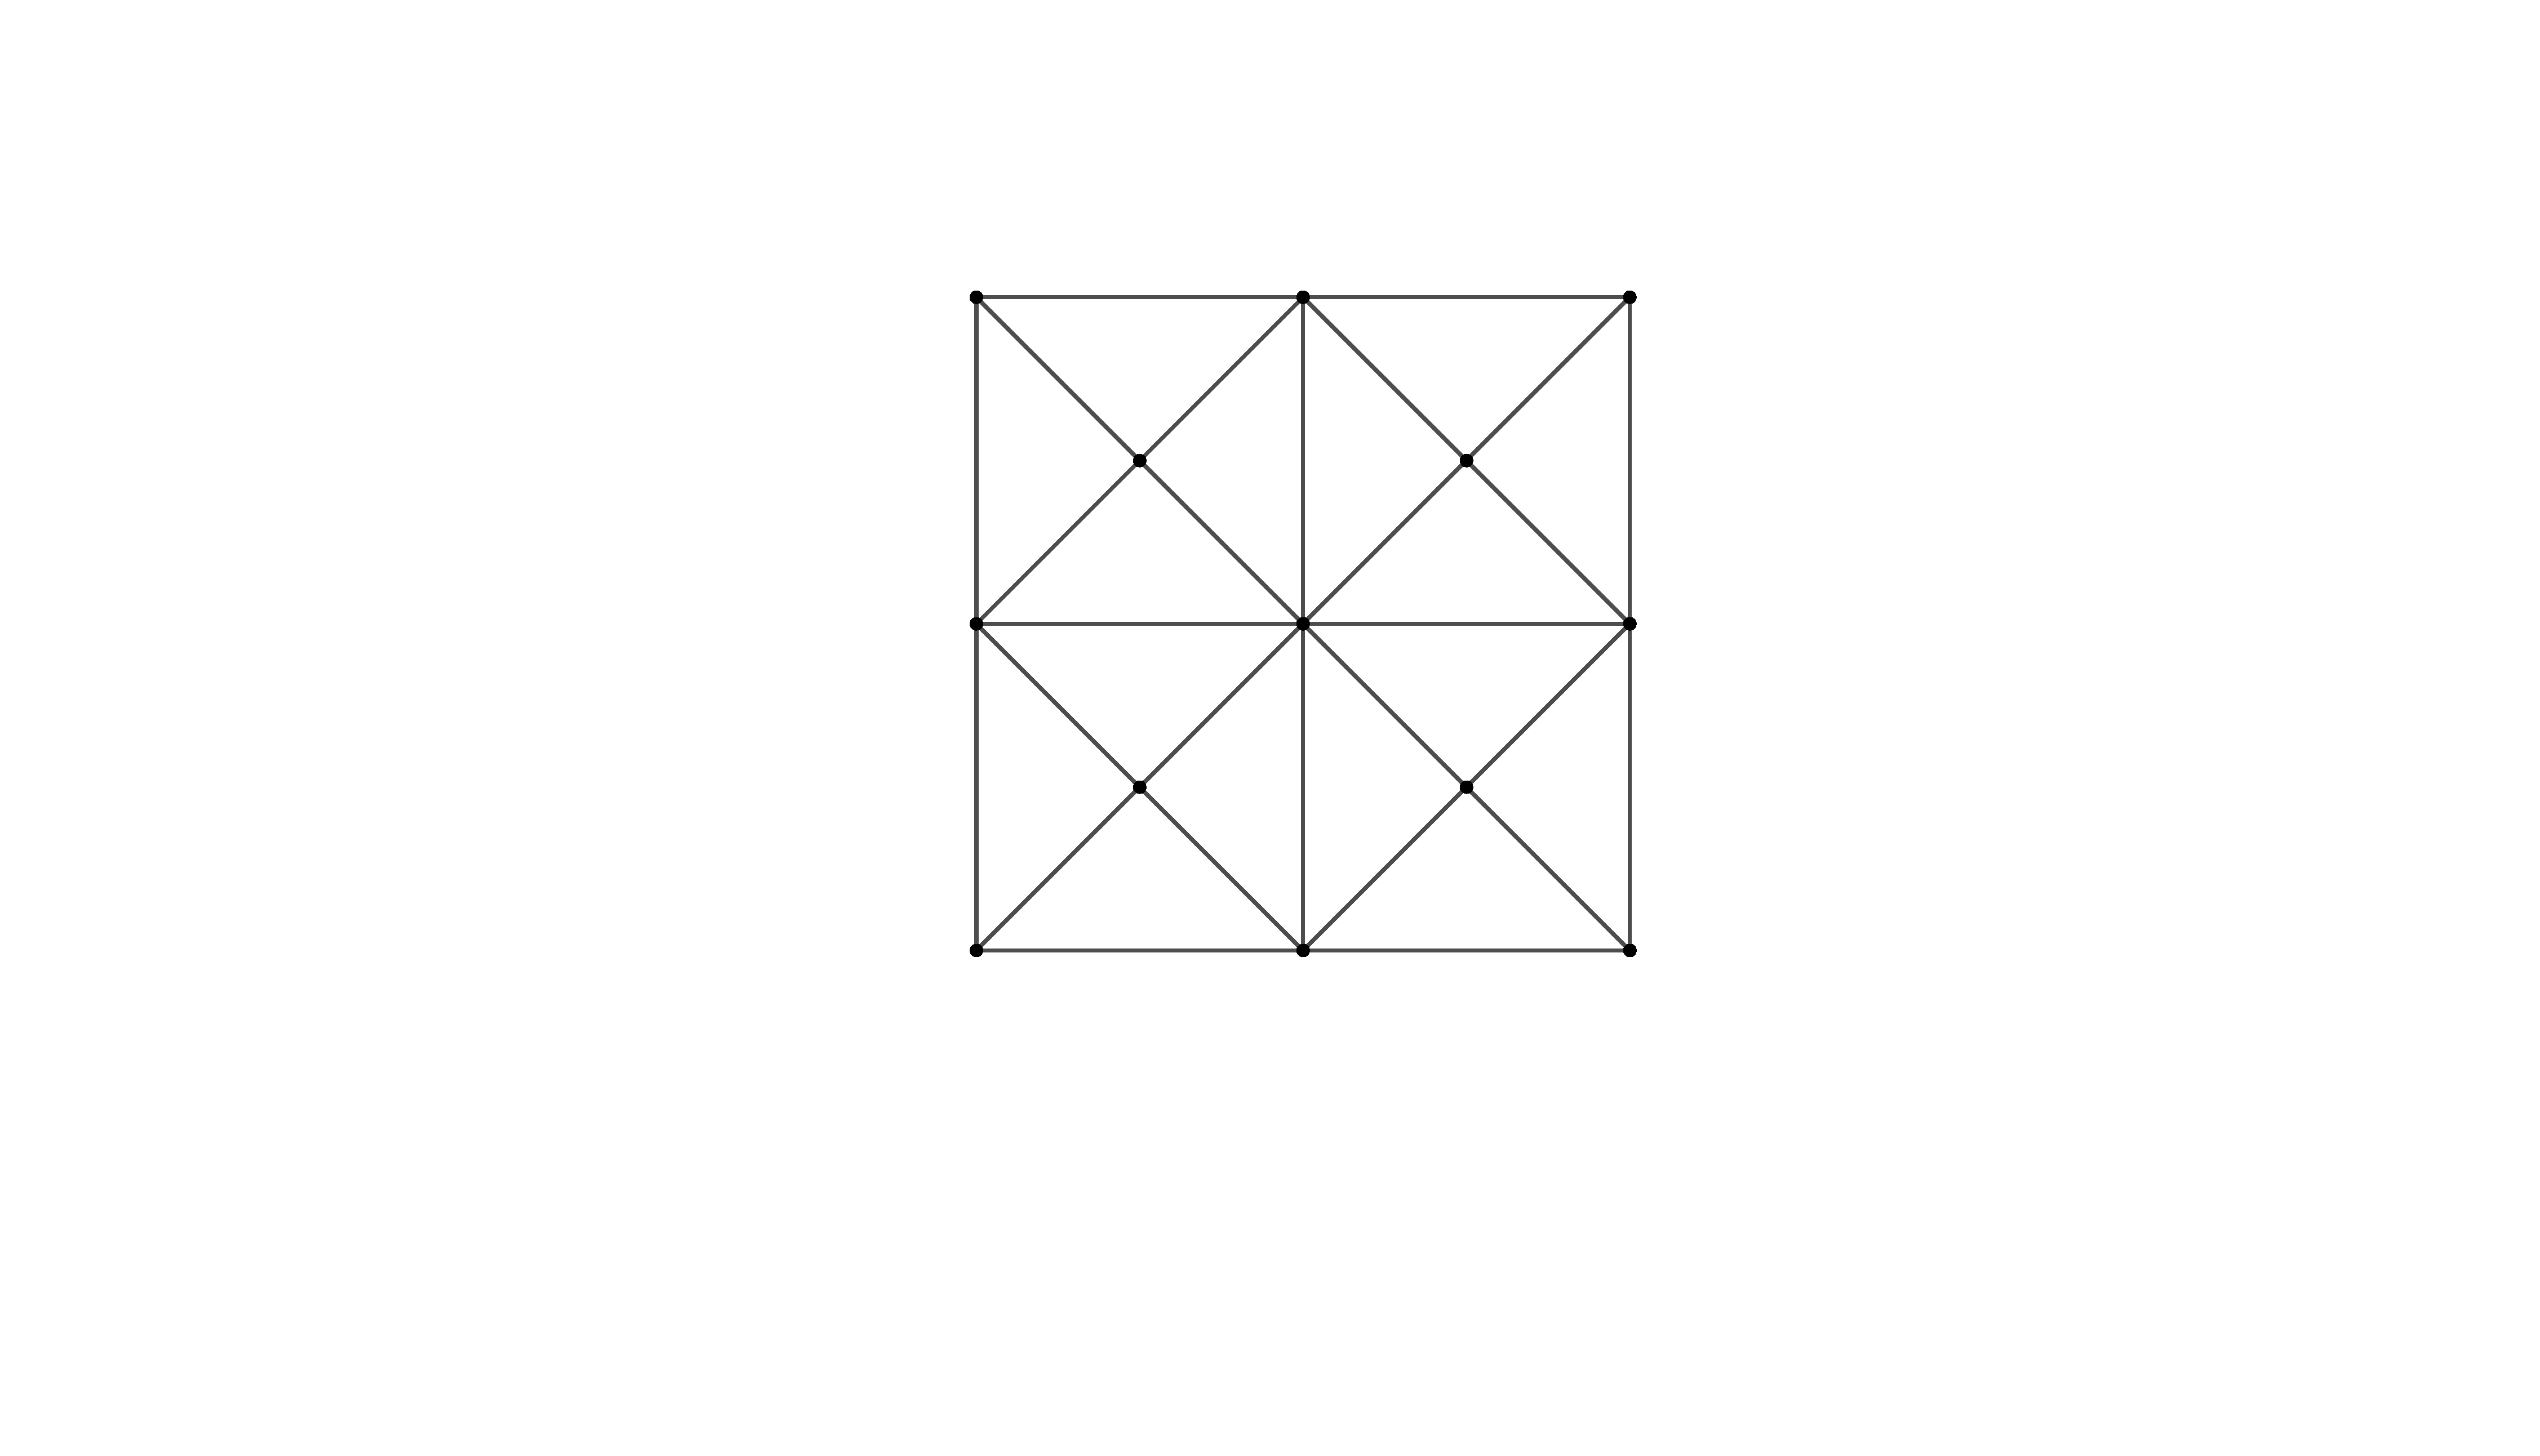
\includegraphics[height=8cm]{discretization.pdf} 
%Example of a mesh with $2$ grid intervals in a cuboid domain.
%\end{center}

Now, let $\mathcal{P}_1(\hat{T}, \mathbb{R})$ be the space of polynomials up to order one in $\hat{T}$. Then, $\{\psi_1, \psi_2, \psi_3\}$ with $\psi_1(\xi)=1-\xi_1-\xi_2$, $\psi_2(\xi)=\xi_1$, $\psi_3(\xi)=\xi_2$ defines a basis of $\mathcal{P}_1(\hat{T}, \mathbb{R})$.
%Therefore, $\{\phi_1, \phi_2, \phi_3\}$ with $\phi_{l_m}= \psi_m \circ \theta_l^{-1}$ for $m=1, 2, 3$ defines a basis of $\mathcal{P}_1(T, \mathbb{R})$.
Using this basis, we set
\begin{displaymath}
%V_h=\{v\in C(\Omega)\mid  v|_{T_l}\in\operatorname*{span}\{\phi_{l_1}, \phi_{l_2}, \phi_{l_3}\}\forall T_l\in\mathcal{T}\}
V_h=\operatorname*{span}\{\phi_i, i=0,\dotsc,N_\mathcal{V}\}\cap V
\end{displaymath}
as the finite element space of our state variables with
\begin{displaymath}
\phi_i|_{T_l}=\begin{cases}
0 & \text{ if $x_i\notin T_l$}\\
\psi_1 \circ \theta_l^{-1} & \text{ if $\theta_l\left(\begin{pmatrix} 0 \\ 0 \end{pmatrix}\right)=x_i$}\\
\psi_2 \circ \theta_l^{-1} & \text{ if $\theta_l\left(\begin{pmatrix} 1 \\ 0 \end{pmatrix}\right)=x_i$}\\
\psi_3 \circ \theta_l^{-1} & \text{ if $\theta_l\left(\begin{pmatrix} 0 \\ 1 \end{pmatrix}\right)=x_i$}
\end{cases} 
\end{displaymath}
for all $T_l\in\mathcal{T}$ and $i=1,\dotsc,N_\mathcal{V}$.

By construction, every $u\in V_h$ is uniquely defined as
\begin{equation}
\label{discretizedUSum}
u=\sum_{i=1}^{N_\mathcal{V}}U_i\phi_i
\end{equation}
with $U_i=u(x_i)$.\\

Now we want to calculate $\int_\Omega u \cdot v \,\mathrm{d}x$ and $\int_\Omega \nabla u \cdot \nabla v \,\mathrm{d}x$ for all $u,v\in  V_h$. In order to do that, we set the mass matrix $\mathbf{M}_n = \left(\int_\Omega \phi_i \cdot \phi_j \,\mathrm{d}x\right)_{i,j=1,\dotsc,N_\mathcal{V}}$ and the stiffness matrix $\mathbf{L}_n = \left(\int_\Omega \nabla\phi_i \cdot \nabla\phi_j \,\mathrm{d}x\right)_{i,j=1,\dotsc,N_\mathcal{V}}$. Let%We calculate these integrals by taking the sum of the integrals over all triangles $T_l\in\mathcal{T}$ where $\phi_i$ and $\phi_j$ are not zero, so all triangles $T_l$ with $x_i,x_j\in T_l$
\begin{displaymath}
\mathbf{U}=\begin{pmatrix} U_1 \\ \vdots \\ U_{N_\mathcal{V}} \end{pmatrix}\text{ and }\mathbf{V}=\begin{pmatrix} V_1 \\ \vdots \\ V_{N_\mathcal{V}} \end{pmatrix},
\end{displaymath}
where $U_i=u(x_i)$, and $V_i=v(x_i)$ for $i=1,\dotsc,N_\mathcal{V}$ as in \eqref{discretizedUSum}. Then we have, based on the representation of elements in $V_h$ from Equation \eqref{discretizedUSum}, that
\begin{displaymath}
\int_\Omega u \cdot v \,\mathrm{d}x=\mathbf{U}^T\mathbf{M}_n\mathbf{V}\text{ and }\int_\Omega \nabla v \cdot \nabla u \,\mathrm{d}x=\mathbf{U}^T\mathbf{L}_n\mathbf{V}.
\end{displaymath}


\subsection{\label{SubsectionDiscretizationInTime}Discretization in time}
For the discretization in time, we first partition the time interval $\bar{I}=[0,T]$ as
\begin{displaymath}
\bar{I}=\{0\}\cup I_1\cup I_2\cup\dotsb\cup I_{N_t}
\end{displaymath}
with subintervals $I_m=(t_{m-1},t_m]$, where $t_m=m\frac{T}{N_t}$ for $m=0,\dotsc, N_t$ and $N_t\in\mathbb{N}$. We want that the discretizations of our functions are continuous in $\bar{I}$ and piecewise polynomial of order one in all subintervals $I_m$, so the discretization space of our state variables is
\begin{displaymath}
X_{k,h}:=\{v\in C(\bar{I},V_h)\mid v |_{I_m}\in\mathcal{P}_1(I_m,V_h),m=1,2,\dotsc,N_t\},
\end{displaymath}
where $\mathcal{P}_1(I_m,V_h)$ denotes the space of polynomials up to order one, defined on $I_m$ with values in $V_h$.
Similarly, we define the time-discretized space of our control variables as
\begin{displaymath}
Q_d:=\{v\in C(\bar{I},H)\mid v |_{I_m}\in\mathcal{P}_1(I_m,H),m=1,2,\dotsc,N_t\}\supset X_{k,h}.
\end{displaymath}

By using the Lagrange basis of $\mathcal{P}_1(I_m,\mathbb{R})$, we can write every functional $v \in Q_d$ as
\begin{equation}
\label{discretizeVariableInTime}
v(t,x)=\left(m-t\frac{N_t}{T}\right) v_{m-1}(x)+\left(t\frac{N_t}{T}-m+1\right) v_m(x)\text{ for }t\in I_m,
\end{equation}
where $v_m(x)=v(t_m,x)$.


\subsection{Crank-Nicolson scheme}
Now we solve the weak state equations \eqref{weakEq} for the state $u\in X_{k,h}$, the control $q\in Q_d$, and $f\in Q$ numerically. Let $u_m=u(t_m, \cdot)$ and $U_{m,i}=u_m(x_i)$ for $m=0,\dotsc,N_t$ and $i=1,\dotsc,N_\mathcal{V}$. We set
\begin{displaymath}
\mathbf{U}_m=\begin{pmatrix} U_{m,1} \\ \vdots \\ U_{m,N_\mathcal{V}} \end{pmatrix}
\end{displaymath}
for $m=0,\dotsc,N_t$. The initial discretized state vector $\mathbf{U}_0$ is already given by the values of $u_0$. Next, we want to solve the weak state equations for $\mathbf{U}_m$ at the other time steps $m=1,\dotsc,N_t$, so that we can set $u_m=\sum_{i=1}^{N_\mathcal{V}}U_{m,i}\phi_i$ according to Equation \eqref{discretizedUSum}.

For this, we find solutions of the Crank-Nicolson scheme \cite{articleMeidner}, so that for $m=1,\dotsc,N_t$ and for all $v\in V_h$:
\begin{eqnarray*}
(u_m,v) + \frac{T}{2N_t}(\nabla u_m, \nabla v) & = &(u_{m-1},v) - \frac{T}{2N_t}(\nabla u_{m-1}, \nabla v)\\
&& + \frac{T}{2N_t}(f_{m-1} + q_{m-1}, v) + \frac{T}{2N_t}(f_m + q_m, v),
\end{eqnarray*}
where $f_m=f(t_m, \cdot)$ and $q_m=q(t_m,\cdot)$. To solve the above equation, while considering the homogeneous Dirichlet boundary conditions, we define the matrix $\tilde{\mathbf{M}}_n\in\mathbb{R}^{N_\mathcal{V}\times N_\mathcal{V}}$ as
%where $u_m$ is a time discretization of $u$ at the time step $t_m$, while $f_m=f(t_m, \cdot)$ and $q_m=q(t_m,\cdot)$. To solve the above equation, we define the matrix $\tilde{\mathbf{M}}_n\in\mathbb{R}^{N_\mathcal{V}\times N_\mathcal{V}}$ as
\begin{displaymath}
\left(\tilde{\mathbf{M}}_n\right)_{i,j}=\begin{cases}
0 & \text{ if $x_i$ or $x_j$ in $\partial\Omega$ and $i \neq j$}\\
1 & \text{ if $x_i$ or $x_j$ in $\partial\Omega$ and $i = j$}\\
\left(\mathbf{M}_n\right)_{i,j} & \text{ else}
\end{cases}
\end{displaymath}
and the matrix $\tilde{\mathbf{L}}_n\in\mathbb{R}^{N_\mathcal{V}\times N_\mathcal{V}}$ as
\begin{displaymath}
\left(\tilde{\mathbf{L}}_n\right)_{i,j}=\begin{cases}
0 & \text{ if $x_j$ in $\partial\Omega$}\\
\left(\mathbf{L}_n\right)_{i,j} & \text{ else,}
\end{cases}
\end{displaymath}
so that $(u_m,v)=\mathbf{U}_m^T\tilde{\mathbf{M}}_n\mathbf{V}$ and $(\nabla u_m,\nabla v)=\mathbf{U}_m^T\tilde{\mathbf{L}}_n\mathbf{V}$ for all $m=0,\dotsc,N_t$, which is giving us
\begin{eqnarray*}
\mathbf{V}^T\tilde{\mathbf{M}}_n^T\mathbf{U}_m + \frac{T}{2N_t} \mathbf{V}^T\tilde{\mathbf{L}}_n^T \mathbf{U}_m &=& \mathbf{V}^T\tilde{\mathbf{M}}_n^T\mathbf{U}_{m-1} - \frac{T}{2N_t} \mathbf{V}^T\tilde{\mathbf{L}}_n^T \mathbf{U}_{m-1}\\
&&  + \frac{T}{2N_t}(f_{m-1} + q_{m-1}, v) + \frac{T}{2N_t}(f_m + q_m, v).
\end{eqnarray*}
In the pyMOR implementation, vectors $\mathbf{F}_m$ for $m=0,\dotsc,N_t$ are defined such that $\mathbf{V}^T\mathbf{F}_m\approx(f_m + q_m, v)$ for all $v\in \mathbf{V}_h$ and $\left(\mathbf{F}_m\right)_i=0$ if the $i$-th entry in the vertex set $\mathcal{V}$ lies on the boundary of $\Omega$. By using these vectors, we get the equation
\begin{equation}
\label{crank_nicolson}
\left(\tilde{\mathbf{M}}_n^T + \frac{T}{2N_t} \tilde{\mathbf{L}}_n^T\right) \mathbf{U}_m = \left(\tilde{\mathbf{M}}_n^T - \frac{T}{2N_t} \tilde{\mathbf{L}}_n^T\right) \mathbf{U}_{m-1} + \frac{T}{2N_t} \mathbf{F}_{m-1} + \frac{T}{2N_t} \mathbf{F}_m,
\end{equation}
which is solved after $\mathbf{U}_m$ with algorithms from the Python package SciPy.

\subsection{\label{subsectionCalculationOfTheObjectiveFunctionValue}Calculation of the objective functional value}
For fixed $\hat{u},f\in Q$, we define $u=u(q)$ for all $q\in Q_d$ so that it satisfies \eqref{crank_nicolson}. The functional value $j(q)$ is now calculated in the following way:
\begin{eqnarray*}
j(q) \approx& \frac{1}{2}\sum_{m=1}^{N_t}\int_{t_{m-1}}^{t_m}&\bigg(\left(m-t\frac{N_t}{T}\right) \left(u_{m-1}-\hat{u}_{m-1}\right)+\left(t\frac{N_t}{T}-m+1\right) \left(u_{m}-\hat{u}_{m}\right),\\
&&\left(m-t\frac{N_t}{T}\right) \left(u_{m-1}-\hat{u}_{m-1}\right)+\left(t\frac{N_t}{T}-m+1\right) \left(u_{m}-\hat{u}_{m}\right)\bigg)\,\mathrm{d}t\\
&+ \frac{\alpha}{2}\sum_{m=1}^{N_t}\int_{t_{m-1}}^{t_m}&\bigg(\left(m-t\frac{N_t}{T}\right) q_{m-1}+\left(t\frac{N_t}{T}-m+1\right) q_{m},\\
&&\left(m-t\frac{N_t}{T}\right) q_{m-1}+\left(t\frac{N_t}{T}-m+1\right) q_{m}\bigg)\,\mathrm{d}t,
\end{eqnarray*}
where $\hat{u}_m=\hat{u}(t_m, \cdot)$. Integration by substitution yields
\begin{eqnarray*}
j(q) \approx& \frac{T}{6N_t}\sum_{m=1}^{N_t}&\left(u_{m-1}-\hat{u}_{m-1},u_{m-1}-\hat{u}_{m-1}\right) + \left(u_{m-1}-\hat{u}_{m-1},u_{m}-\hat{u}_{m}\right)\\
&&+ \left(u_{m}-\hat{u}_{m},u_{m}-\hat{u}_{m}\right)\\
&+ \frac{\alpha T}{6N_t}\sum_{m=1}^{N_t}&\left(q_{m-1},q_{m-1}\right) + \left(q_{m-1},q_{m}\right) + \left(q_{m},q_{m}\right)\\
\approx& \frac{T}{6N_t}\sum_{m=1}^{N_t}&\left(\mathbf{U}_{m-1}-\hat{\mathbf{U}}_{m-1}\right)\mathbf{M}_n\left(\mathbf{U}_{m-1}-\hat{\mathbf{U}}_{m-1}\right)\\
&&+ \left(\mathbf{U}_{m-1}-\hat{\mathbf{U}}_{m-1}\right)\mathbf{M}_n\left(\mathbf{U}_{m}-\hat{\mathbf{U}}_{m}\right)\\
&&+ \left(\mathbf{U}_{m}-\hat{\mathbf{U}}_{m}\right)\mathbf{M}_n\left(\mathbf{U}_{m}-\hat{\mathbf{U}}_{m}\right)\\
&+ \frac{\alpha T}{6N_t}\sum_{m=1}^{N_t}&\mathbf{Q}_{m-1}\mathbf{M}_n\mathbf{Q}_{m-1} + \mathbf{Q}_{m-1}\mathbf{M}_n\mathbf{Q}_{m} + \mathbf{Q}_{m}\mathbf{M}_n\mathbf{Q}_{m},
\end{eqnarray*}
where $\hat{\mathbf{U}}_m=\left(\hat{u}(t_m, x_i)\right)_{i=1,\dotsc,N_\mathcal{V}}$ and $\mathbf{Q}_m=\left(q(t_m, x_i)\right)_{i=1,\dotsc,N_\mathcal{V}}$ for $m=0,\dotsc,N_t$.

\section{Optimization of the control variable}

In our optimization procedure, we search for a control variable among all elements $q\in Q_d$ which are defined by using a fixed set of $N_b\in\mathbb{N}$ shape functionals
\begin{equation}
\label{basisFuncionsList}
\Phi=\{\phi_1,\dotsc,\phi_{N_b}\}
\end{equation}
 with $\phi_1,\dotsc,\phi_{N_b}\in H$ and scalars $q_1^0,q_1^1,\dotsc,q_1^{N_t},\dotsc,q_{N_b}^0,q_{N_b}^1\dotsc,q_{N_b}^{N_t}\in\mathbb{R}$, as a linear combination of the shape functionals in $\Phi$ with time-dependent factors. That is
\begin{equation}
\label{discrContrVar}
q(t,x) = \sum_{i=1}^{N_b}\alpha_i(t)\phi_i(x),
\end{equation} 
where the factors $\alpha_i(t)$ are for $t\in I_m$ a weighted sum between $q^{m-1}_i$ and $q^m_i$ with $m=1,\dotsc,N_t$ as in \eqref{discretizeVariableInTime}:
\begin{displaymath}
\alpha_i(t)=\begin{cases}
q_i^{m-1}\left(m-t\frac{N_t}{T}\right) + q_i^m\left(t\frac{N_t}{T}-m+1\right) & \text{ if $t\in I_m$ with $m=1,\dotsc,N_t$}\\
q_i^0 & \text{ if $t=0$.}
\end{cases}
\end{displaymath}
Each control variable that is written in this form can be represented by a control vector
\begin{displaymath}
\mathbf{q}=\left[q_1^0,q_1^1,\dotsc,q_1^{N_t},\dotsc,q_{N_b}^0,q_{N_b}^1\dotsc,q_{N_b}^{N_t}\right]^T\in\mathcal{D},
\end{displaymath} 
where $\mathcal{D}:=\mathbb{R}^{N_\mathbf{q}}$ with $N_\mathbf{q} = (N_t+1)\cdot N_b$ is the domain of this vector. Hence, we write
\begin{equation}
\label{FOMFunctionalEvaluationDef}
j(\mathbf{q}):=j(q)
\end{equation}
for each $q$ that is defined like in \eqref{discrContrVar}. In the remaining chapters, we want to find a $\mathbf{q}\in\mathcal{D}$ that minimizes this functional. That is
\begin{equation}
\label{FOMOptimizationProblemDef}
\operatorname*{minimize}_{\mathbf{q}\in\mathcal{D}}j(\mathbf{q}).
\end{equation}

In this thesis, we refer to evaluations of the functional $j$ in \eqref{FOMFunctionalEvaluationDef} with
\begin{equation*}
\begin{aligned}
j(q)=\frac{T}{6N_t}\sum_{m=1}^{N_t}&\left(\mathbf{U}_{m-1}-\hat{\mathbf{U}}_{m-1}\right)\mathbf{M}_n\left(\mathbf{U}_{m-1}-\hat{\mathbf{U}}_{m-1}\right)\\
&+ \left(\mathbf{U}_{m-1}-\hat{\mathbf{U}}_{m-1}\right)\mathbf{M}_n\left(\mathbf{U}_{m}-\hat{\mathbf{U}}_{m}\right)\\
&+ \left(\mathbf{U}_{m}-\hat{\mathbf{U}}_{m}\right)\mathbf{M}_n\left(\mathbf{U}_{m}-\hat{\mathbf{U}}_{m}\right)\\
+ \frac{\alpha T}{6N_t}\sum_{m=1}^{N_t}&\mathbf{Q}_{m-1}\mathbf{M}_n\mathbf{Q}_{m-1} + \mathbf{Q}_{m-1}\mathbf{M}_n\mathbf{Q}_{m} + \mathbf{Q}_{m}\mathbf{M}_n\mathbf{Q}_{m},
\end{aligned}
\end{equation*}
as full order model (FOM) functional evaluations. The optimization problem in \eqref{FOMOptimizationProblemDef} is called the FOM optimization problem. In the next chapters, we present algorithms that solve the FOM optimization problem. Thus, the FOM functional is also the objective functional.
































































